%% EE588 AWG Project Presentation  ── v2 (updated with N=24 results)
%% 10-minute talk, 15 slides
%% Compile:  pdflatex EE588_AWG_Presentation.tex  (run twice)
%%
%% FIGURE PLACEMENT QUICK-REFERENCE (all paths relative to this .tex file):
%%   Slide  6  right col : results/figures/neff_vs_width.png
%%   Slide  7  right col : results/figures/simplified_awg_geometry_layout.png
%%   Slide  8  right col : results/figures/awg_transmission_spectra.png
%%   Slide 10  right col : results/figures/awg_high_fidelity_transmission.png
%%   Slide 11  left col  : results/figures/awg_hf_optimization_scan.png
%%   Slide 12  right col : results/figures/awg_improved_design_channels.png  ← NEW
%%   Slide 14  bottom    : results/figures/awg_hf_global_optimization_channels.png
%%
%% See the companion file  EE588_AWG_图片放置指南.md  for exact placements.

\documentclass[aspectratio=169,10pt]{beamer}

% ── Theme ─────────────────────────────────────────────────────────────────────
\usetheme{Madrid}
\usecolortheme{seahorse}
\setbeamertemplate{navigation symbols}{}
\setbeamertemplate{footline}[frame number]

% ── Packages ──────────────────────────────────────────────────────────────────
\usepackage{graphicx}
\usepackage{booktabs}
\usepackage{amsmath}
\usepackage{xcolor}
\usepackage{tikz}
\usepackage{array}
\usepackage{multirow}
\usepackage{hyperref}

% ── Colors ────────────────────────────────────────────────────────────────────
\definecolor{uw_purple}{RGB}{51,0,111}
\definecolor{uw_gold}{RGB}{232,211,162}
\definecolor{good_green}{RGB}{0,153,76}
\definecolor{passing_blue}{RGB}{0,102,204}
\definecolor{poor_red}{RGB}{204,0,0}
\setbeamercolor{frametitle}{bg=uw_purple,fg=white}
\setbeamercolor{title}{bg=uw_purple,fg=white}
\setbeamercolor{structure}{fg=uw_purple}

% ── Metadata ──────────────────────────────────────────────────────────────────
\title[EE588 AWG Project]{C-band 4-Channel AWG Wavelength Demultiplexer\\
       Design \& Simulation using Tidy3D}
\subtitle{EE588 Final Project}
\author{Jiahua Luo}
\institute{University of Washington}
\date{\today}

% ─────────────────────────────────────────────────────────────────────────────
\begin{document}

% ════════════════════════════════════════════════════════════════════════════
%  SLIDE 1 — Title
% ════════════════════════════════════════════════════════════════════════════
\begin{frame}
  \titlepage
\end{frame}

% ════════════════════════════════════════════════════════════════════════════
%  SLIDE 2 — Motivation I: The Data Center Bandwidth Challenge
% ════════════════════════════════════════════════════════════════════════════
\begin{frame}{Motivation I: The Data Center Bandwidth Challenge}
  \begin{columns}[T]
    \column{0.55\textwidth}
      \textbf{Global IP traffic is exploding}
      \begin{itemize}
        \item Data-center IP traffic reached \textbf{20.6 ZB/year} in 2021,
              growing $\sim$25\% annually \footnotemark[1]
        \item 77\% of all traffic stays \emph{inside} data centers
              (intra-DC communications)
        \item Scaling with more copper wires hits fundamental limits:
              resistance, crosstalk, energy per bit
      \end{itemize}

      \vspace{0.6em}
      \textbf{Optical interconnects are the answer}
      \begin{itemize}
        \item 400GbE / 800GbE standards now mandate WDM optics \footnotemark[2]
        \item \textbf{WDM}: multiplex $N$ wavelength channels on a single fiber
        \item Receiver side needs a \textbf{wavelength demultiplexer (demux)}
              to separate channels
      \end{itemize}

    \column{0.42\textwidth}
      \begin{block}{The core challenge}
        \centering
        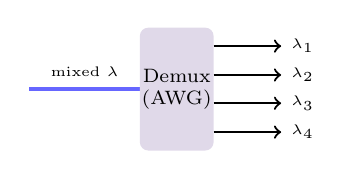
\begin{tikzpicture}[scale=0.78, font=\small]
          % fiber
          \draw[very thick, blue!60] (-1.8,0) -- (0,0);
          \node[above] at (-0.9,0.05) {\tiny mixed $\lambda$};
          % demux box
          \fill[uw_purple!15, rounded corners=3pt] (0,-1.0) rectangle (1.2,1.0);
          \node[align=center, font=\scriptsize] at (0.6,0) {Demux\\(AWG)};
          % output channels
          \foreach \y/\lbl in {0.7/$\lambda_1$, 0.23/$\lambda_2$,
                                -0.23/$\lambda_3$, -0.7/$\lambda_4$}{
            \draw[thick, ->] (1.2,\y) -- (2.3,\y)
              node[right, font=\tiny] {\lbl};
          }
        \end{tikzpicture}
        \vspace{0.4em}\\
        One fiber in, four color-separated channels out.
        \textbf{This is what we build.}
      \end{block}
  \end{columns}

  \footnotetext[1]{\tiny Cisco Annual Internet Report 2018–2023, White Paper, 2022.}
  \footnotetext[2]{\tiny D. A. B. Miller, ``Rationale and challenges for optical interconnects,''
    \textit{Proc.\ IEEE}, vol.\ 88, pp.\ 728--749, 2000.}
\end{frame}

% ════════════════════════════════════════════════════════════════════════════
%  SLIDE 3 — Motivation II: Why Silicon AWG?
% ════════════════════════════════════════════════════════════════════════════
\begin{frame}{Motivation II: Why Arrayed Waveguide Grating on Silicon?}
  \begin{columns}[T]
    \column{0.50\textwidth}
      \textbf{AWG: the dominant on-chip demux architecture}
      \begin{itemize}
        \item First proposed by Smit (1988) \footnotemark[3]; now found in
              virtually every coherent transceiver
        \item Operates as a \emph{phased-array spatial filter}: $N$ waveguide
              arms with incremental path-length difference $\Delta L$ produce
              wavelength-dependent constructive interference
        \item Channel count 4–96, insertion loss $<$\,2 dB in state-of-the-art
              Si implementations \footnotemark[4]
      \end{itemize}

      \vspace{0.5em}
      \textbf{Why silicon (SOI platform)?}
      \begin{itemize}
        \item CMOS-compatible: fab in existing semiconductor foundries
        \item Large index contrast Si/SiO$_2$ ($\Delta n \approx 2.0$)
              $\Rightarrow$ sub-micron waveguide, mm$^2$ footprint
        \item Integrates with Ge photodetectors and Si modulators
              on the same chip \footnotemark[5]
      \end{itemize}

    \column{0.47\textwidth}
      \begin{block}{ITU-T C-band channel plan \footnotemark[6]}
        \centering
        \renewcommand{\arraystretch}{1.1}
        \begin{tabular}{cc}
          \toprule
          Channel & Center $\lambda$ (nm) \\
          \midrule
          ch\,1 & 1547.6 \\
          ch\,2 & 1549.2 \\
          ch\,3 & 1550.8 \\
          ch\,4 & 1552.4 \\
          \midrule
          \multicolumn{2}{c}{$\Delta\lambda = 1.6$\,nm $\approx$ 200\,GHz} \\
          \bottomrule
        \end{tabular}
      \end{block}
      \vspace{0.3em}
      \small\textit{This project}: simulate this exact 4-channel plan on a
      500\,nm\,$\times$\,220\,nm Si strip waveguide platform.
  \end{columns}

  \footnotetext[3]{\tiny M. K. Smit, ``New focusing and dispersive planar component based on an optical phased array,''
    \textit{Electron.\ Lett.}, vol.\ 24, pp.\ 385--386, 1988.}
  \footnotetext[4]{\tiny M. K. Smit \& C. van Dam, ``PHASAR-based WDM-devices,''
    \textit{IEEE JSTQE}, vol.\ 2, pp.\ 236--250, 1996.}
  \footnotetext[5]{\tiny L. Chrostowski \& M. Hochberg, \textit{Silicon Photonics Design},
    Cambridge Univ.\ Press, 2015.}
  \footnotetext[6]{\tiny ITU-T G.694.1, ``DWDM frequency grid,'' 2012.}
\end{frame}

% ════════════════════════════════════════════════════════════════════════════
%  SLIDE 4 — AWG Working Principle
% ════════════════════════════════════════════════════════════════════════════
\begin{frame}{AWG Working Principle: Phased-Array Interference}
  \begin{center}
  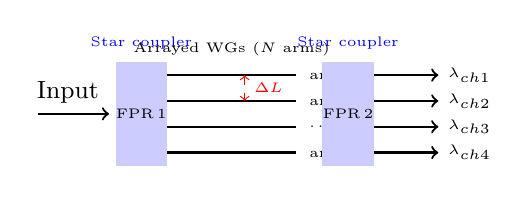
\begin{tikzpicture}[scale=0.82, every node/.style={font=\small}]
    \draw[thick,->] (-1.2,0) -- (-0.1,0) node[above left]{\small Input};
    \fill[blue!20] (0,-0.8) rectangle (0.8,0.8);
    \node at (0.4,0) {\tiny FPR\,1};
    \foreach \y/\lbl in {0.6/arm\,0, 0.2/arm\,1, -0.2/\ldots, -0.6/arm\,N\!-\!1}{
      \draw[thick] (0.8,\y) -- (2.8,\y);
      \node[right] at (2.85,\y) {\tiny \lbl};
    }
    \draw[<->,dashed,red] (2.0,0.6) -- (2.0,0.2) node[midway,right]{\tiny $\Delta L$};
    \fill[blue!20] (3.2,-0.8) rectangle (4.0,0.8);
    \node at (3.6,0) {\tiny FPR\,2};
    \foreach \y/\ch in {0.6/ch1, 0.2/ch2, -0.2/ch3, -0.6/ch4}{
      \draw[thick,->] (4.0,\y) -- (5.0,\y);
      \node[right] at (5.0,\y) {\tiny $\lambda_{\ch}$};
    }
    \node[above,blue] at (0.4,0.85) {\tiny Star coupler};
    \node[above,blue] at (3.6,0.85) {\tiny Star coupler};
    \node[above] at (1.8,0.75) {\tiny Arrayed WGs ($N$ arms)};
  \end{tikzpicture}
  \end{center}

  \begin{columns}[T]
    \column{0.50\textwidth}
      \textbf{Key design equations:}
      \[
        \Delta L = \frac{m\,\lambda_0}{n_g}, \quad
        \text{FSR} = \frac{\lambda_0}{m}, \quad
        \text{3dB BW} \approx \frac{\text{FSR}}{N}
      \]
      \small Phase of arm $k$ at wavelength $\lambda$:
      $\phi_k = \dfrac{2\pi\,n_\text{eff}(\lambda)}{\lambda}\cdot k\Delta L$

    \column{0.47\textwidth}
      \begin{block}{This project's parameters}
        \small
        $m=81$,\quad $\Delta L \approx 30.99\,\mu$m,\quad FSR $\approx 19.1$\,nm\\[3pt]
        \textbf{Initially} $N=16$: 3dB BW $= 1.2$\,nm\\
        \textbf{Improved} $N=24$: 3dB BW $= 0.8$\,nm\\[3pt]
        Channel spacing $= 1.6$\,nm $>$ BW \checkmark
      \end{block}
  \end{columns}
\end{frame}

% ════════════════════════════════════════════════════════════════════════════
%  SLIDE 5 — Simulation Strategy
% ════════════════════════════════════════════════════════════════════════════
\begin{frame}{Three-Level Simulation Strategy}
  \begin{center}
  \renewcommand{\arraystretch}{1.35}
  \begin{tabular}{clll}
    \toprule
    \textbf{Level} & \textbf{Method} & \textbf{What it answers} & \textbf{Cost} \\
    \midrule
    1 & Tidy3D MODE solver & Waveguide $n_\text{eff}$, $n_g$ & $\sim$0.006 FC/run \\
    2 & Local array-factor model & Ideal spectrum shape & \textbf{Free} \\
    3 & Tidy3D 2D eff.-index FDTD & Real EM routing in FPR & $\sim$0.10 FC/run \\
    \rowcolor{gray!15}
    (4) & Full 3D FDTD (not done) & Accurate IL \& XT & $\sim$7.8 FC/run \\
    \bottomrule
  \end{tabular}
  \end{center}

  \vspace{0.4em}
  \begin{columns}[T]
    \column{0.50\textwidth}
      \begin{block}{2D effective-index shortcut}
        Replace 3D waveguide with 2D medium at $n = n_\text{eff}$.
        Model only the output-FPR section; inject phased
        sources to represent the array arms analytically.\\[3pt]
        Savings: $\sim$100$\times$ vs full 3D.
      \end{block}

    \column{0.47\textwidth}
      \begin{alertblock}{Total project cost}
        \small
        MODE runs: $\sim$0.03 FC\\
        Level-3 FDTD (36 runs): $\sim$3.2 FC\\
        \textbf{Grand total: $\approx$\,3.2 FlexCredit}\\[2pt]
        Full-3D equivalent: $> 300$ FC
      \end{alertblock}
  \end{columns}
\end{frame}

% ════════════════════════════════════════════════════════════════════════════
%  SLIDE 6 — Waveguide MODE Analysis
%  📷 RIGHT COL: results/figures/neff_vs_width.png
% ════════════════════════════════════════════════════════════════════════════
\begin{frame}{Phase 1 — Waveguide MODE Analysis}
  \begin{columns}[T]
    \column{0.44\textwidth}
      \textbf{Si strip / SiO$_2$ clad:} $h = 220$\,nm (fixed SOI)\\[0.4em]
      \begin{tabular}{ccc}
        \toprule
        Width & $n_\text{eff}$ & $n_g$ \\
        \midrule
        400\,nm & 2.228 & 4.245 \\
        450\,nm & 2.353 & 4.144 \\
        \rowcolor{uw_gold!60}
        \textbf{500\,nm}$^\star$ & \textbf{2.445} & \textbf{4.051} \\
        550\,nm & 2.513 & 3.975 \\
        600\,nm & 2.566 & 3.914 \\
        \bottomrule
      \end{tabular}
      \vspace{0.5em}

      \small$^\star$ Selected: mid-range, single-mode, standard SOI width.\\[0.4em]
      \textbf{Trends:} wider $w$ $\Rightarrow$ $n_\text{eff}\uparrow$ (better confinement),
      $n_g\downarrow$ (weaker dispersion).\\[0.4em]
      $n_g$ enters directly into $\Delta L = m\lambda_0/n_g$.

    \column{0.53\textwidth}
      \begin{center}
        % 📷 FILE: results/figures/neff_vs_width.png
        % Dual-axis plot: n_eff (left) and n_group (right) vs waveguide width
        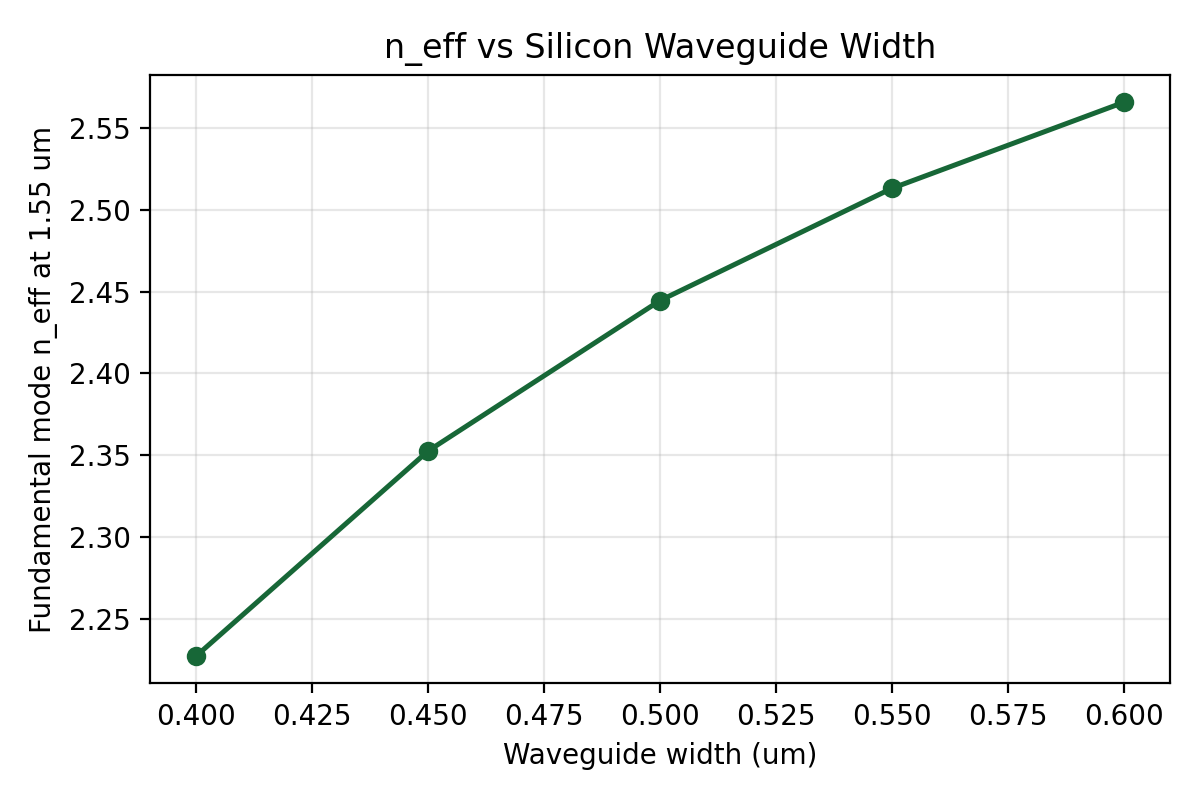
\includegraphics[width=\linewidth]{results/figures/neff_vs_width.png}
        \footnotesize $n_\text{eff}$ and $n_g$ vs.\ width at 1550\,nm
      \end{center}
  \end{columns}
\end{frame}

% ════════════════════════════════════════════════════════════════════════════
%  SLIDE 7 — AWG Design Parameters + Geometry
%  📷 RIGHT COL: results/figures/simplified_awg_geometry_layout.png
% ════════════════════════════════════════════════════════════════════════════
\begin{frame}{Phase 2 — AWG Initial Design}
  \begin{columns}[T]
    \column{0.44\textwidth}
      \textbf{Design derivation chain:}
      \renewcommand{\arraystretch}{1.15}
      \begin{tabular}{ll}
        \toprule
        Parameter & Value \\
        \midrule
        Center $\lambda_0$ & 1550\,nm \\
        $\Delta\lambda$ & 1.6\,nm \\
        Target FSR & 19.2\,nm \\
        AWG order $m$ & 81 \\
        Actual FSR & 19.14\,nm \\
        $\Delta L = m\lambda_0/n_g$ & 30.99\,$\mu$m \\
        \midrule
        Input / output / arms & 1 / 4 / 16 \\
        FPR length & 55\,$\mu$m \\
        Array pitch (init.) & 1.50\,$\mu$m \\
        Output pitch (init.) & 2.00\,$\mu$m \\
        \bottomrule
      \end{tabular}

    \column{0.53\textwidth}
      \begin{center}
        % 📷 FILE: results/figures/simplified_awg_geometry_layout.png
        % Top-view schematic: 1 input, FPR1, 16 array arms, FPR2, 4 outputs
        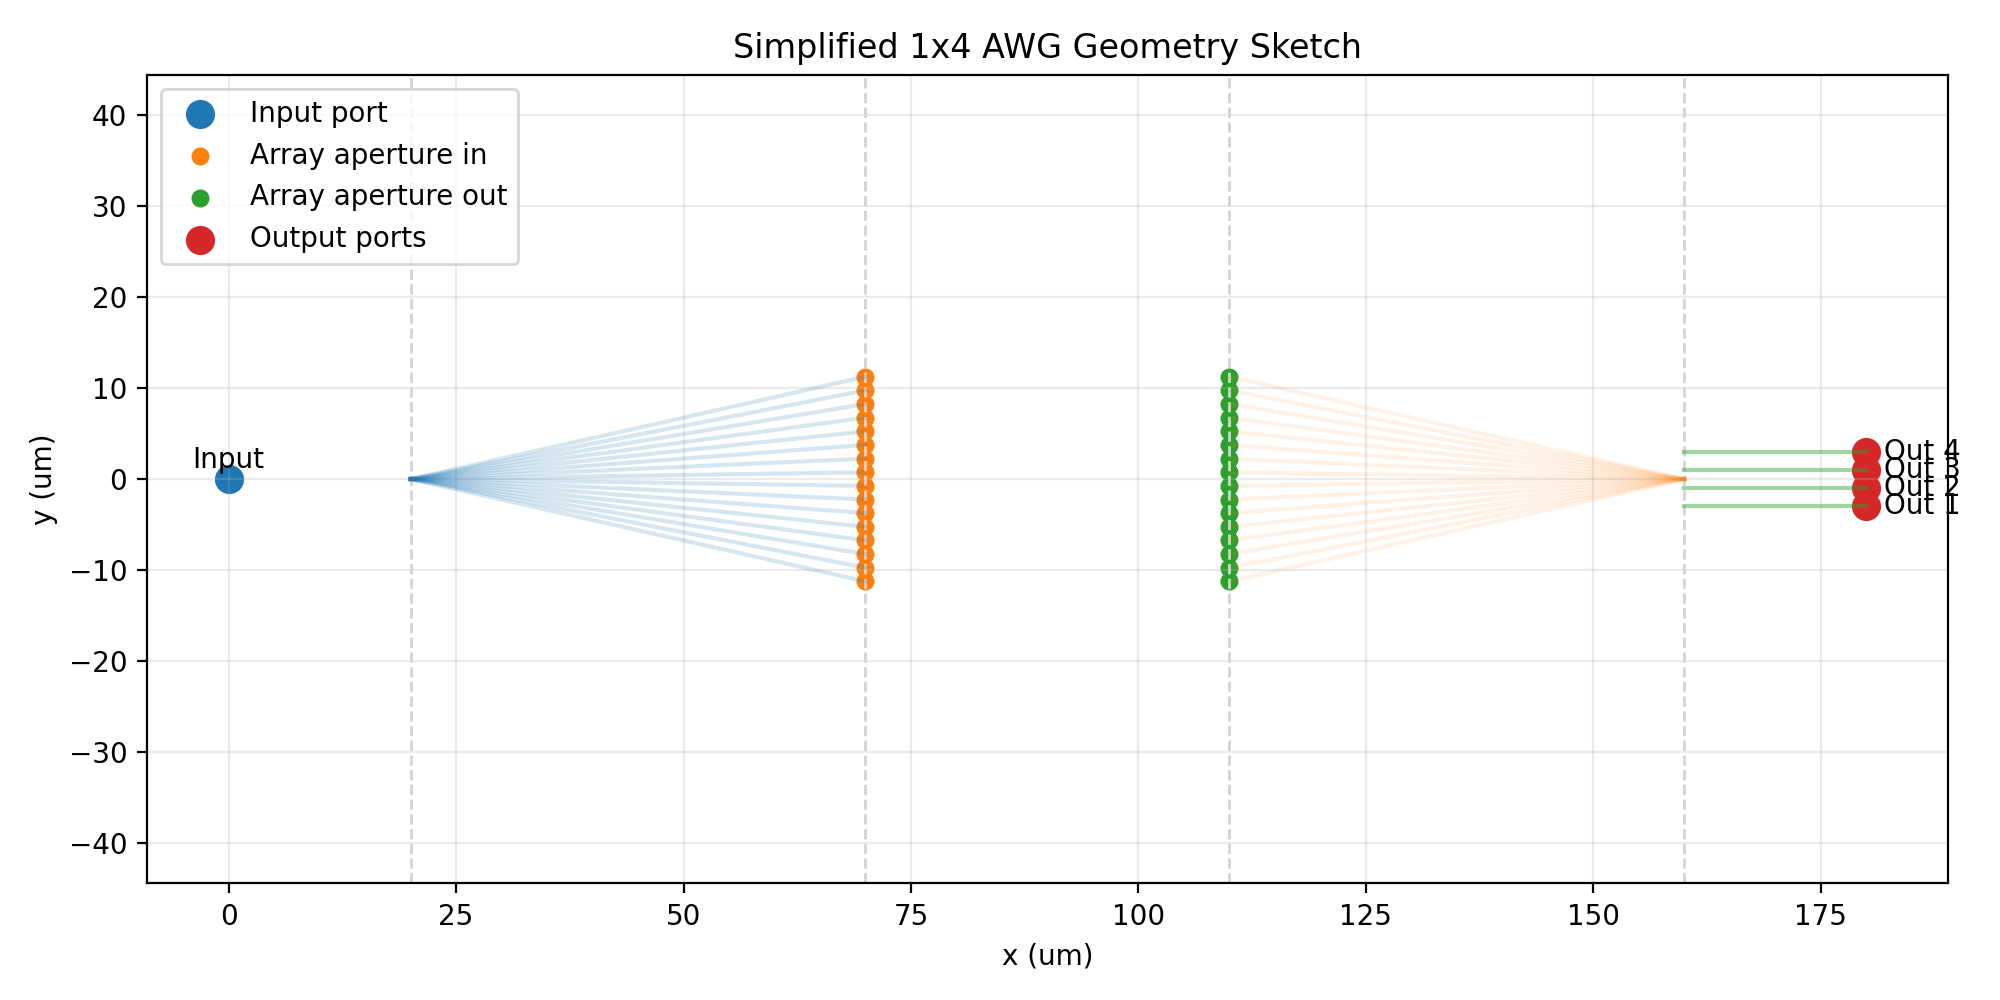
\includegraphics[width=\linewidth]{results/figures/simplified_awg_geometry_layout.png}
        \footnotesize Simplified AWG layout: 1 input, 4 outputs, 16 arms
      \end{center}
  \end{columns}
\end{frame}

% ════════════════════════════════════════════════════════════════════════════
%  SLIDE 8 — Simplified Spectrum Model
%  📷 RIGHT COL: results/figures/awg_transmission_spectra.png
% ════════════════════════════════════════════════════════════════════════════
\begin{frame}{Phase 3a — Array-Factor Spectrum Model (Zero Cloud Cost)}
  \begin{columns}[T]
    \column{0.44\textwidth}
      \textbf{Analytic model:}
      \[
        T(\lambda) = T_\text{pk} \cdot
        \underbrace{\!\left(\frac{\sin(N\phi/2)}{N\sin(\phi/2)}\right)^{\!2}}_{\text{array factor}}
        \cdot
        \underbrace{e^{-\delta\lambda^2/2\sigma^2}}_{\text{envelope}}
      \]
      $\phi = 2\pi\delta\lambda/\text{FSR}$,\quad$N=16$,\quad$\sigma=6$\,nm.

      \vspace{0.6em}
      \begin{block}{Predicted channel metrics}
        \small
        \begin{tabular}{ll}
          Insertion loss & 3.0\,dB \\
          Crosstalk      & $-$13.7\,dB \\
          3\,dB BW       & 1.06\,nm \\
          Ch.\ spacing   & 1.60\,nm\,\checkmark \\
        \end{tabular}
      \end{block}

      \begin{alertblock}{\small Limitation}
        \small Symmetric model: all 4 channels identical.
        Real device: edge channels have higher IL.
      \end{alertblock}

    \column{0.53\textwidth}
      \begin{center}
        % 📷 FILE: results/figures/awg_transmission_spectra.png
        % Overlaid transmission vs wavelength for all 4 channels
        % Shows 4 peaks at 1547.6 / 1549.2 / 1550.8 / 1552.4 nm
        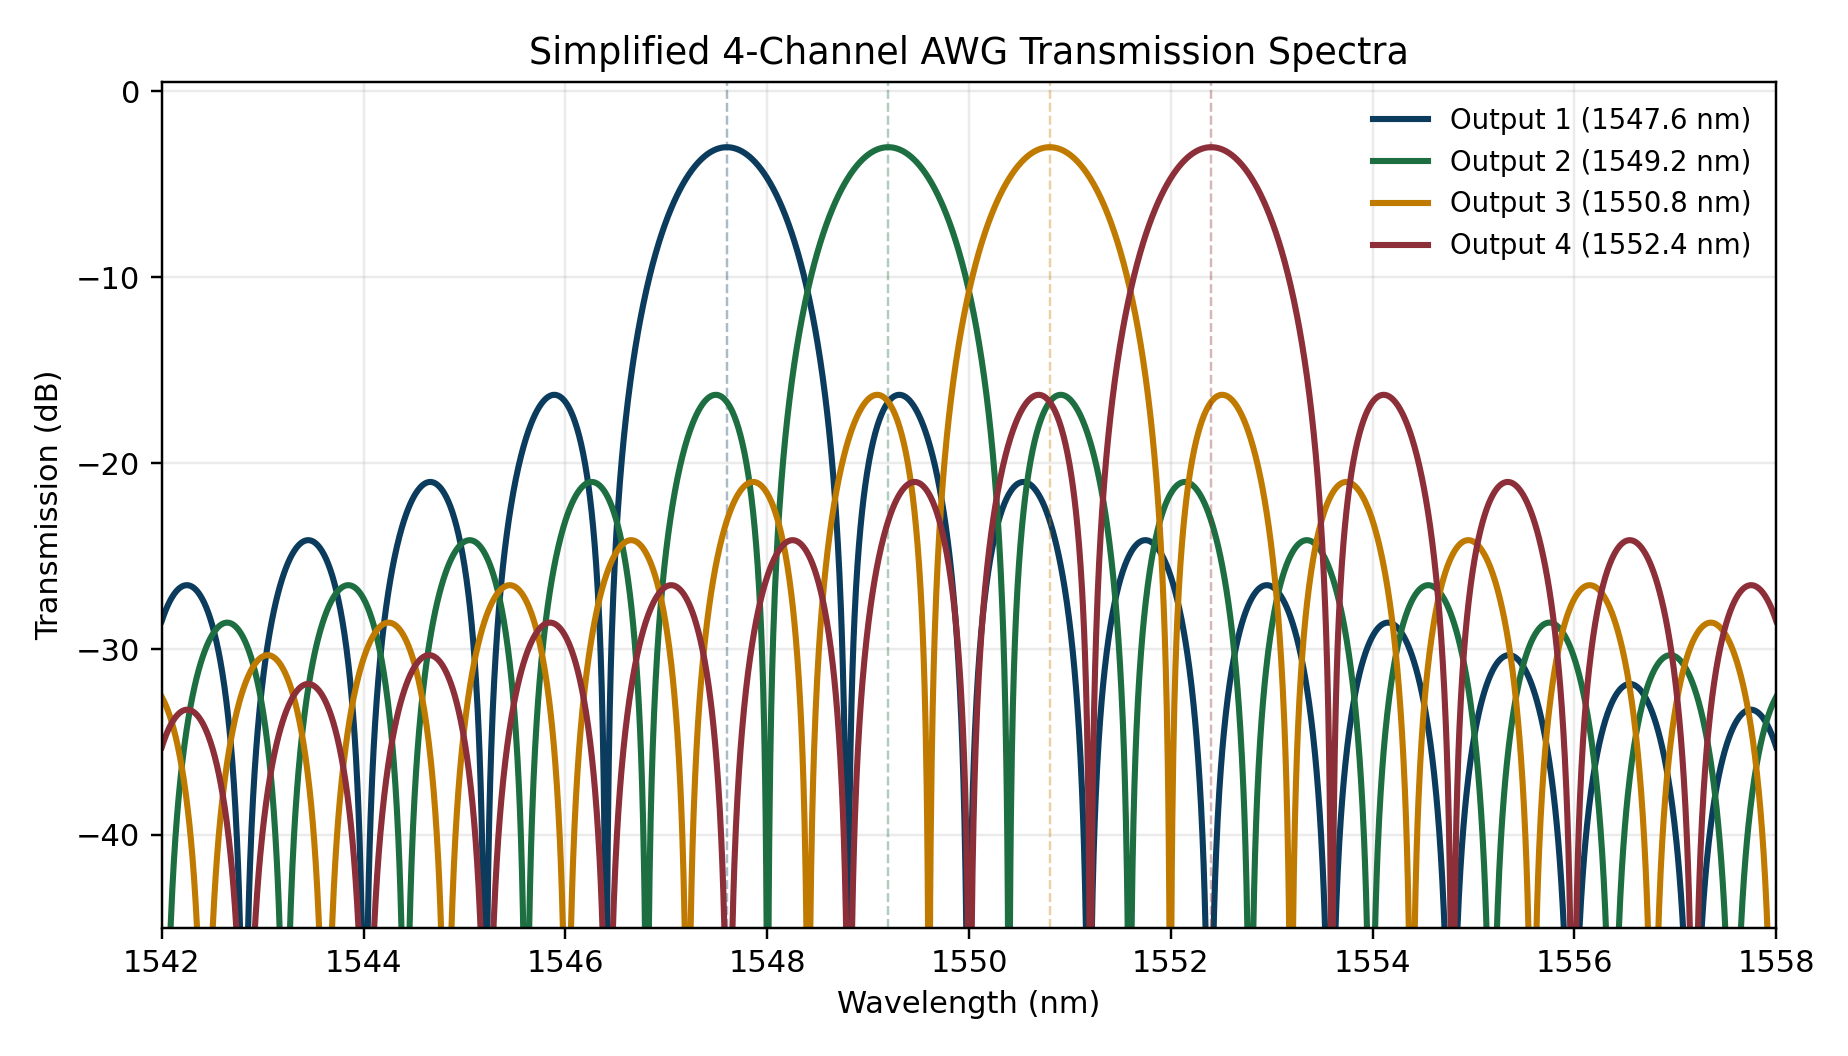
\includegraphics[width=\linewidth]{results/figures/awg_transmission_spectra.png}
        \footnotesize Predicted 4-channel transmission spectrum
      \end{center}
  \end{columns}
\end{frame}

% ════════════════════════════════════════════════════════════════════════════
%  SLIDE 9 — FDTD Validation Setup & Rubric
% ════════════════════════════════════════════════════════════════════════════
\begin{frame}{Phase 3b — High-Fidelity 2D FDTD Validation}
  \begin{columns}[T]
    \column{0.50\textwidth}
      \textbf{2D eff.-index FDTD model:}
      \begin{itemize}
        \item Explicitly models: phased-array aperture + FPR slab + output WGs
        \item Arm phases set analytically: $\varphi_k = \beta k\Delta L$
              (avoids the 2\,mm-scale arm meanders)
        \item $\sim$0.10 FC/run vs $\sim$7.8 FC for full 3D
        \item Total: $\approx$36 FDTD runs, $\approx$3.2 FC
      \end{itemize}

    \column{0.47\textwidth}
      \textbf{Routing quality rubric:}
      \renewcommand{\arraystretch}{1.2}
      \begin{tabular}{lcc}
        \toprule
        Grade & Dom.\ frac. & 2nd/1st \\
        \midrule
        \textcolor{good_green}{\textbf{Good}}      & $\geq 0.60$ & $\leq 0.50$ \\
        \textcolor{passing_blue}{\textbf{General}} & $\geq 0.40$ & $\leq 0.80$ \\
        \textbf{Passing}                           & $\geq 0.30$ & $\leq 0.95$ \\
        \textcolor{poor_red}{\textbf{Poor}}        & \multicolumn{2}{c}{below passing} \\
        \bottomrule
      \end{tabular}
      \vspace{0.4em}\\
      \footnotesize
      \textit{Dom.\ frac.} $=$ strongest port / total flux.\\
      \textit{2nd/1st} $=$ 2nd / strongest (lower = cleaner).
  \end{columns}
\end{frame}

% ════════════════════════════════════════════════════════════════════════════
%  SLIDE 10 — Baseline FDTD Results
%  📷 RIGHT COL: results/figures/awg_high_fidelity_transmission.png
% ════════════════════════════════════════════════════════════════════════════
\begin{frame}{Baseline FDTD — Wavelength Routing Confirmed}
  \begin{columns}[T]
    \column{0.44\textwidth}
      \textbf{Config: } $N=16$, pitch $= 1.5\,\mu$m, out-pitch $= 2.0\,\mu$m
      \renewcommand{\arraystretch}{1.2}
      \begin{tabular}{cccc}
        \toprule
        $\lambda$ & Dom. & Dom.\ frac & Grade \\
        \midrule
        1547.6 & out\_3 & 0.390 & Passing \\
        1549.2 & out\_3 & 0.340 & Passing \\
        1550.8 & out\_4 & 0.328 & Passing \\
        1552.4 & out\_4 & 0.350 & Passing \\
        \midrule
        \textbf{Avg} & — & \textbf{0.352} & Passing \\
        \bottomrule
      \end{tabular}

      \vspace{0.5em}
      \begin{block}{Key finding}
        Dominant output shifts out\_3 $\to$ out\_4 as $\lambda$ increases.\\[3pt]
        \textbf{Wavelength-dependent routing confirmed}
        in real FDTD — not just analytic prediction.
      \end{block}

    \column{0.53\textwidth}
      \begin{center}
        % 📷 FILE: results/figures/awg_high_fidelity_transmission.png
        % 4-panel bar chart: output flux at each port for each of the 4 wavelengths
        % Dominant bar shifts from out_3 to out_4 across wavelengths
        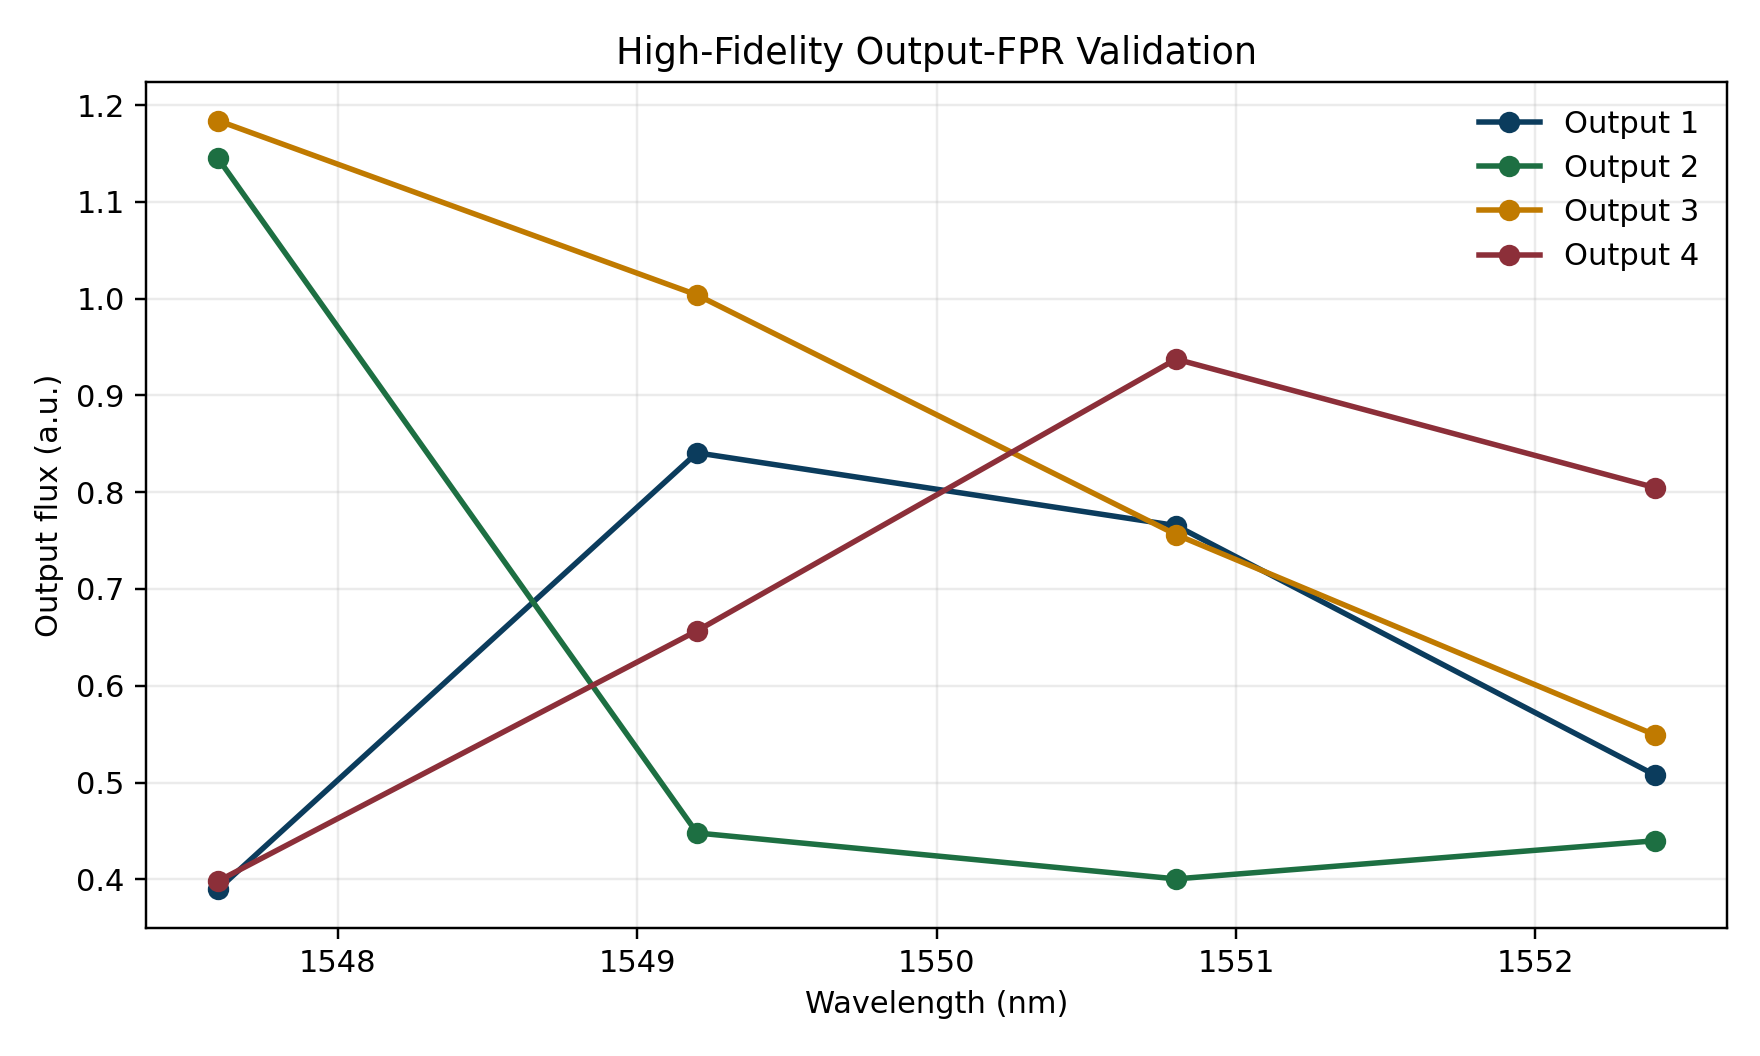
\includegraphics[width=\linewidth]{results/figures/awg_high_fidelity_transmission.png}
        \footnotesize Output flux per port at each wavelength (baseline)
      \end{center}
  \end{columns}
\end{frame}

% ════════════════════════════════════════════════════════════════════════════
%  SLIDE 11 — Optimization Journey (3 rounds, N=16)
%  📷 LEFT COL: results/figures/awg_hf_optimization_scan.png
% ════════════════════════════════════════════════════════════════════════════
\begin{frame}{Optimization Journey — Rounds 1–3 (N\,=\,16)}
  \begin{columns}[T]
    \column{0.49\textwidth}
      \begin{center}
        % 📷 FILE: results/figures/awg_hf_optimization_scan.png
        % Bar chart: dominant fraction for 9 scanned configs at 1550.8 nm
        % Shows optscan_c as clear winner (general quality)
        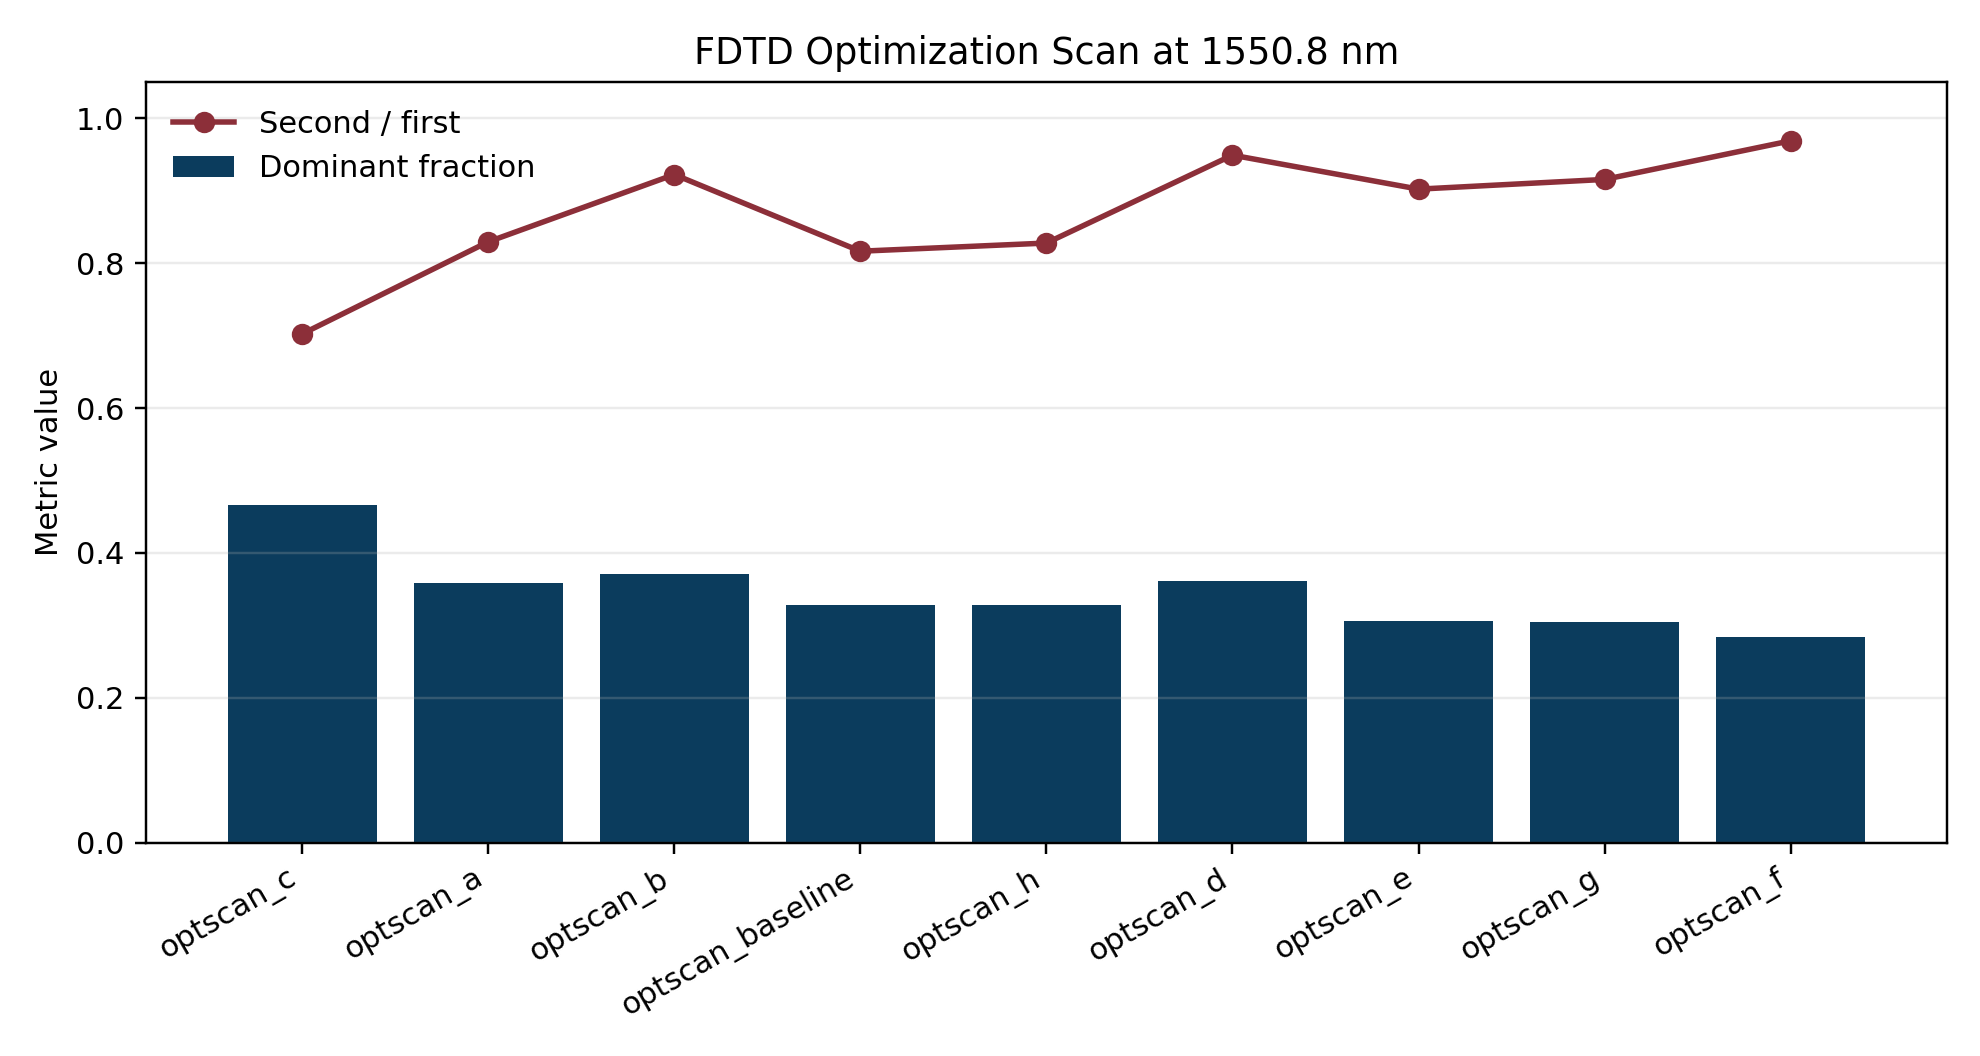
\includegraphics[width=\linewidth]{results/figures/awg_hf_optimization_scan.png}
        \footnotesize Round-2 scan at 1550.8\,nm: 9 configs
      \end{center}

    \column{0.49\textwidth}
      \textbf{Progression of average dom.\ fraction:}
      \renewcommand{\arraystretch}{1.25}
      \begin{tabular}{lcc}
        \toprule
        Round & Config & Avg dom.\ frac \\
        \midrule
        Baseline     & 1.5/2.0/0.0   & 0.352 \\
        R1: coarse   & 375-pt scan   & (screening) \\
        R2: local    & 1.2/1.6/0.6   & 0.368 \\
        R3: global   & 1.2/1.6/0.6   & 0.368 \\
        \bottomrule
      \end{tabular}

      \vspace{0.5em}
      \small\textbf{Best N=16 config} (R2/R3):\\
      array pitch $= 1.20\,\mu$m,
      out pitch $= 1.60\,\mu$m,
      offset $= 0.60\,\mu$m\\[4pt]
      1550.8\,nm: Passing $(0.328)$ $\to$ \textbf{General} $(0.466)$\\[2pt]
      \textbf{Bottleneck}: 3dB BW $= 1.2$\,nm $\approx$ channel spacing $1.6$\,nm.
      Adjacent channels overlap heavily.
  \end{columns}
\end{frame}

% ════════════════════════════════════════════════════════════════════════════
%  SLIDE 12 — Key Improvement: N=24 Arms  ← NEW
%  📷 RIGHT COL: results/figures/awg_improved_design_channels.png
% ════════════════════════════════════════════════════════════════════════════
\begin{frame}{Key Improvement — Increasing Array Arm Count to N\,=\,24}
  \begin{columns}[T]
    \column{0.44\textwidth}
      \textbf{Physical insight:} 3dB BW $= $ FSR$/N$
      \begin{itemize}
        \item $N=16$: BW $= 1.2$\,nm — only $0.75\times$ channel spacing
        \item $N=24$: BW $= 0.8$\,nm — $0.5\times$ channel spacing
        \item Aperture $= 16 \times 1.2 = 19.2\,\mu$m $\to$
              $24 \times 1.2 = 28.8\,\mu$m (fits in 34\,$\mu$m slab)
        \item Cost increase: negligible (same simulation domain)
      \end{itemize}

      \vspace{0.5em}
      \textbf{Best new config} (\textit{impr\_C}):
      $N=24$, pitch $= 1.2\,\mu$m,
      out-pitch $= 1.8\,\mu$m, offset $= 0.9\,\mu$m

      \renewcommand{\arraystretch}{1.15}
      \begin{tabular}{cccc}
        \toprule
        $\lambda$ & Dom. & Dom.\ frac & Grade \\
        \midrule
        1547.6 & out\_3 & \textbf{0.473} & \textcolor{passing_blue}{\textbf{General}} \\
        1549.2 & out\_3 & \textbf{0.419} & \textcolor{passing_blue}{\textbf{General}} \\
        1550.8 & out\_1 & 0.307 & Passing \\
        1552.4 & out\_3 & \textbf{0.414} & Passing \\
        \midrule
        \textbf{Avg} & — & \textbf{0.403} & — \\
        \bottomrule
      \end{tabular}

    \column{0.53\textwidth}
      \begin{center}
        % 📷 FILE: results/figures/awg_improved_design_channels.png
        % 4-panel grouped bar chart comparing configs A/B/C/D (N=24)
        % Each panel = one config, bars = 4 output ports at 4 wavelengths
        % impr_C panel shows out_3 consistently dominant
        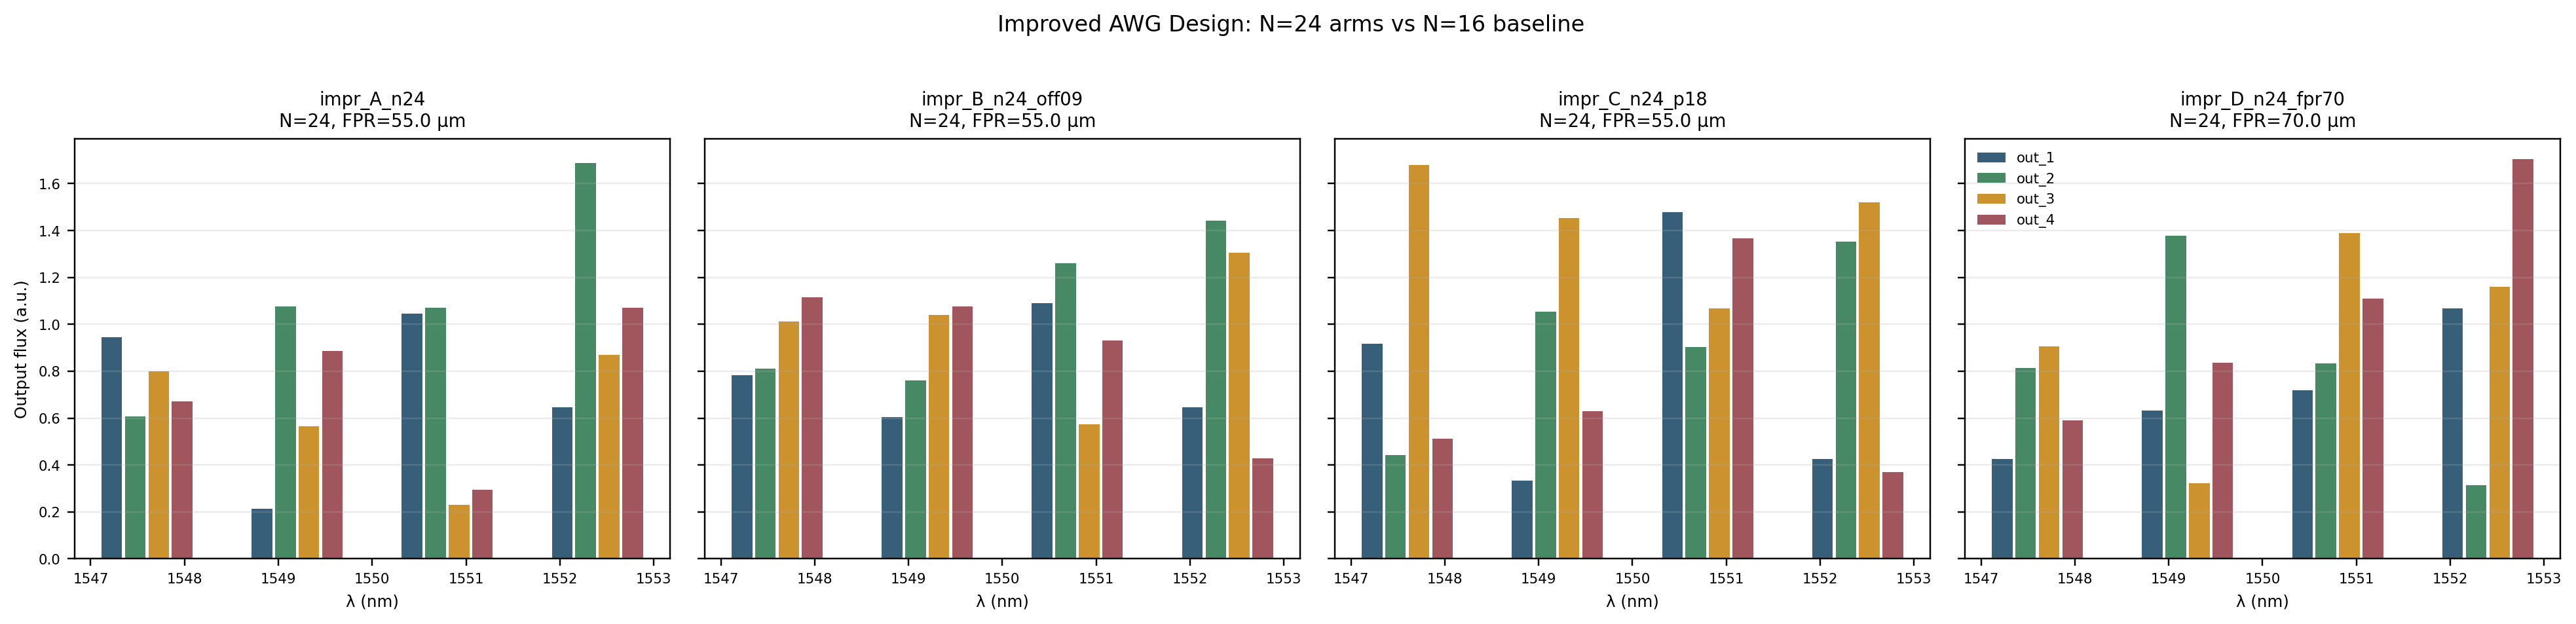
\includegraphics[width=\linewidth]{results/figures/awg_improved_design_channels.png}
        \footnotesize N=24 configs: 4 output ports × 4 wavelengths each
      \end{center}
  \end{columns}
\end{frame}

% ════════════════════════════════════════════════════════════════════════════
%  SLIDE 13 — Stretch Goals
% ════════════════════════════════════════════════════════════════════════════
\begin{frame}{Stretch Goals — Preliminary FDTD Results}
  \begin{columns}[T]
    \column{0.32\textwidth}
      \begin{block}{8-Channel Extension}
        \small
        8-output layout, pitch $= 1.3\,\mu$m\\[0.3em]
        At 1550\,nm: dominant $=$ \textbf{out\_7} \checkmark\\[0.3em]
        Proves workflow scales beyond 4 channels without redesign.
      \end{block}

    \column{0.32\textwidth}
      \begin{block}{Thermal Sensitivity}
        \small
        Modeled $+40$\,K via thermo-optic effect\\
        $dn/dT = 1.86\!\times\!10^{-4}$\,K$^{-1}$\\[0.3em]
        Dominant output shifts from out\_4 $\to$ \textbf{out\_2}\\[0.3em]
        Confirms AWG thermal drift: real devices need TEC or athermal design.
      \end{block}

    \column{0.32\textwidth}
      \begin{block}{Crosstalk Reduction}
        \small
        Best N=16 config (1.2/1.6/0.6):\\[0.3em]
        \begin{tabular}{ll}
          Baseline: & 0.328 \\
          Optimized: & \textbf{0.466} \\
        \end{tabular}\\[0.3em]
        $+42\%$ at center $\lambda$.
        Further gain via Rowland-circle FPR geometry.
      \end{block}
  \end{columns}
\end{frame}

% ════════════════════════════════════════════════════════════════════════════
%  SLIDE 14 — Complete Results Summary
% ════════════════════════════════════════════════════════════════════════════
\begin{frame}{Complete Optimization Results Summary}
  \begin{center}
  \renewcommand{\arraystretch}{1.35}
  \begin{tabular}{llcccc}
    \toprule
    \textbf{Round} & \textbf{Config} & \textbf{Avg dom.} & \textbf{General ch.} &
    \textbf{Max 2nd/1st} & \textbf{Cost (FC)} \\
    \midrule
    Baseline & N=16, 1.5/2.0/0.0 & 0.352 & 0 & 0.967 & 0.30 \\
    R1 coarse screen & 375 local sims & — & — & — & 0 \\
    R2 local opt & N=16, 1.2/1.6/0.6 & 0.368 & 1 & 0.932 & 0.67 \\
    R3 global opt & N=16, 1.2/1.6/0.6 & 0.368 & 1 & 0.932 & 0.52 \\
    \rowcolor{uw_gold!50}
    \textbf{R4 N=24} & \textbf{N=24, 1.2/1.8/0.9} & \textbf{0.403} &
    \textbf{2} & \textbf{0.924} & \textbf{1.66} \\
    \bottomrule
  \end{tabular}
  \end{center}

  \vspace{0.3em}
  \begin{columns}[T]
    \column{0.48\textwidth}
      \textbf{Cumulative improvement (Baseline $\to$ R4):}
      \begin{itemize}
        \item Avg dom.\ frac: $0.352 \to \mathbf{0.403}$ \quad ($+15$\%)
        \item Channels reaching General: $0 \to \mathbf{2}$
        \item Max 2nd/1st: $0.967 \to \mathbf{0.924}$
      \end{itemize}

    \column{0.48\textwidth}
      \textbf{Key lesson:} adjusting geometry alone (R2/R3) gave modest gain.
      Changing the \emph{physics} — more arms reduce 3dB BW —
      was the single most effective move (\textbf{R4}).
  \end{columns}
\end{frame}

% ════════════════════════════════════════════════════════════════════════════
%  SLIDE 15 — Conclusions
% ════════════════════════════════════════════════════════════════════════════
\begin{frame}{Conclusions \& Future Work}
  \begin{columns}[T]
    \column{0.50\textwidth}
      \textbf{Accomplished:}
      \begin{enumerate}
        \item MODE sweep: $n_g = 4.051$ for 500\,nm Si WG
        \item AWG design: $m=81$, $\Delta L = 30.99\,\mu$m
        \item Array-factor model: IL $= 3$\,dB, XT $= -13.7$\,dB
        \item FDTD validation: wavelength routing \textbf{proven}
        \item 3 rounds of geometry opt: \textbf{center $\lambda$} General
        \item N=24 redesign: \textbf{2 channels} General ($+15$\% avg)
        \item Stretch goals: 8-ch, thermal, XT improvement
      \end{enumerate}

    \column{0.47\textwidth}
      \textbf{Remaining limitations:}
      \begin{itemize}
        \item Full 4-channel set not yet all-General
        \item 1550.8\,nm center channel weakens in N=24 config \\
              \small(flat FPR geometry causes asymmetric focusing)
        \item 2D model ignores bend loss, mode mismatch
      \end{itemize}

      \vspace{0.5em}
      \textbf{Next steps (priority order):}
      \begin{enumerate}\small
        \item Fine-tune N=24 offset ($\sim$0.3 FC)
        \item \textbf{Rowland-circle FPR} — fix center-ch anomaly
        \item N=32 + FPR=90\,$\mu$m ($\sim$0.5 FC)
        \item Full 3D FDTD for accurate IL/XT
      \end{enumerate}
  \end{columns}

  \vspace{0.6em}
  \begin{center}
    \large\textbf{Thank you!} \quad Questions?
  \end{center}
\end{frame}

\end{document}
